% !TEX root = ../Yan Hao--Dissertation.tex

\chapter{Questions on the Central Level}
% Fiscal federalism is a form of fiscal decentralization that is widely recognized as a more efficient way to provide public goods and services, particularly in large and complex countries with multiple levels of administrative institutions. Hayek \cite{hayek2009use} argued that local governments are better positioned to understand local needs and preferences, and therefore to provide appropriate public goods and services. Stigler \cite{stigler1998tenable} built on Hayek's insights and argued for the necessity of protecting the funding ability of subnational governments. Tiebout \cite{tiebout1956pure} developed a theoretical framework to show that voting with one's feet can ensure that public goods supply matches local needs. He also demonstrated that competition among local governments can lead to improved administrative efficiency. Tiebout's theory seems get supported by the actual data showed in Table \ref*{Table 2.1}, which potentially reflects the difference of tax burden preference of different states. These foundational insights form the basis for much of the research on the advantages of fiscal federalism. For the following part, I'll focus on the evaluation of decentralized fiscal structure which is fiscal federalism.


% % Table generated by Excel2LaTeX from sheet 'Sheet1'
% \begin{table}[H]
%     \centering
%     \caption{Effective Tax Revenue in America}
%     \begin{tabular}{p{9.43em}lll}
%         \toprule
%         State                & \multicolumn{1}{p{8.145em}}{State and Local Taxes (\$ billions)} & \multicolumn{1}{p{7.43em}}{Personal Income (\$ billions)} & \multicolumn{1}{p{9.93em}}{Effective Tax Rate} \\
%         \midrule
%         New York             & \multicolumn{1}{c}{177.8}                                        & \multicolumn{1}{c}{1,281.10}                              & \multicolumn{1}{c}{13.90\%}                    \\
%         District of Columbia & \multicolumn{1}{c}{7.5}                                          & \multicolumn{1}{c}{55.5}                                  & \multicolumn{1}{c}{13.40\%}                    \\
%         North Dakota         & \multicolumn{1}{c}{5}                                            & \multicolumn{1}{c}{39.5}                                  & \multicolumn{1}{c}{12.70\%}                    \\
%         Hawaii               & \multicolumn{1}{c}{9.5}                                          & \multicolumn{1}{c}{75.4}                                  & \multicolumn{1}{c}{12.60\%}                    \\
%         Vermont              & \multicolumn{1}{c}{3.8}                                          & \multicolumn{1}{c}{32.6}                                  & \multicolumn{1}{c}{11.70\%}                    \\
%         \midrule
%         United States Total  & \multicolumn{1}{c}{1,652.80}                                     & \multicolumn{1}{c}{16,820.30}                             & \multicolumn{1}{c}{9.80\%}                     \\
%         \midrule
%         Alabama              & \multicolumn{1}{c}{16.4}                                         & \multicolumn{1}{c}{198.9}                                 & \multicolumn{1}{c}{8.30\%}                     \\
%         Oklahoma             & \multicolumn{1}{c}{13.9}                                         & \multicolumn{1}{c}{174.4}                                 & \multicolumn{1}{c}{8.00\%}                     \\
%         \midrule
%         \multicolumn{4}{p{34.935em}}{\textit{Source:U.S. Census Bureau Dataset}}                                                                                                                             \\
%     \end{tabular}%
%     \label{Table 2.1}%
% \end{table}%


% \section{How to Evaluate the Fiscal Federalism System}
% Even within the topic of fiscal federalism, the fiscal federalism structures in different countries have different content and features, needless to say, they show different impact in public goods and services supplying. Like I mentioned in Chapter 1, it's hard and nearly impossible to find a perfect stick yard criterion to compare fiscal federalism in different countries. I'll try to explain and get a comprehensive way to evaluate fiscal federalism. Literature about fiscal federalism can be roughly divided into two groups. First-generation theory of fiscal federalism concentrate on the fiscal structure itself, focusing on the efficiency of federalism in collecting revenue and offering responsibilities, and whether the revenue-responsibility combination perform well in public goods supply. Coming to second-generation theory of fiscal federalism, scholars get interested in the effect of fiscal federalism on other area such as the effect on economic development.

% \subsection{First-Generation Theory of Fiscal Federalism}

% Evaluating the efficiency of fiscal structures is a common approach to assessing their reasonableness. Pareto efficiency, which requires that resources be allocated in a manner that cannot make anyone better off without making someone else worse off, is widely accepted as a standard for evaluation \cite{pareto2014manual}. Scholars have identified three economic factors useful in evaluating fiscal structures: externalities, information complexity, and incentive compatibility. Oates \cite{oates1972fiscal} proposed that governments and residents of a jurisdiction should bear the costs of negative externalities and receive payment for positive externalities. Olson \cite{olson1993dictatorship} argued that the "free rider" problem could be resolved by making jurisdictions and beneficiary areas identical, achieving an equilibrium in which marginal costs equal marginal benefits. One example of an efficiency consideration in the United States' fiscal federalism structure is the revenue structure for individual taxes, as shown in Table \ref*{Table 2.2}. To minimize behavioral distortions and improve efficiency, individual income taxes, which are easy to move across jurisdictions, are mainly collected by federal and state governments, allowing individuals to be indifferent about where they live and pay taxes.

% % Table generated by Excel2LaTeX from sheet 'Sheet1'
% \begin{table}[htbp]
%     \centering
%     \caption{. Percentage Composition of Tax Revenue by Government Level}
%     \begin{tabular}{lccc}
%         \toprule
%         \multicolumn{1}{c}{Type} & Federal & State   & Local   \\
%         \midrule
%         Individual income        & 51.80\% & 37.20\% & 4.70\%  \\
%         Corporate income         & 6.90\%  & 4.70\%  & 1.10\%  \\
%         Other taxes              & 41.20\% & 58.10\% & 94.20\% \\
%         \bottomrule
%     \end{tabular}%
%     \label{Table 2.2}%
% \end{table}%


% Besides, information complexity is an important consideration in evaluating fiscal federalism structure. Basing their work on the earlier contributions of Hayek and Tiebout, Bseley et al \cite{2003Centralized} developed a political economy model to simulate the decision-making process in a democratic country. They emphasized the advantage of local government in public goods supplying and introduced insensitivity of central government into their model. Information communication is also important, with local governments having better knowledge of local residents' needs and their behavior being better perceived by local residents. Decentralized fiscal federalism structures put local governments under supervision, as noted by Dethier \cite{martinez2003fiscal} and based on Tiebout's voting on feet framework. Baicker \cite{baicker2005spillover} introduced a horizontal competition structure with multiple local governments and states that enables local residents to evaluate local governments' efficiency in public goods supply under a yardstick competition framework. This information transparency can push local governments to improve their performance.

% Finally, a well-designed fiscal structure should satisfy the criterion of incentive compatibility. Incentive compatibility is a game theory concept introduced by Leonid Hurwicz \cite{hurwicz1973design} that requires a mechanism to be designed such that each participant can achieve the best outcome for themselves by acting truthfully. In public administration and public economics, incentive compatibility has become an important criterion for evaluating the quality of fiscal federalism. Proper fiscal federalism settings can motivate local governments to efficiently provide public goods. For example, Eckstein \cite{eckstein1958water} argues that the proper combination of funding resources and responsibilities can motivate organizations, including local governments, to work hard and provide public goods efficiently, since working hard with efficiency in public goods supplying is an weakly dominate strategy and could attract more residents and increase more public funding resource. Under the impact of incentive compatibility theory, scholars generally assume that local governments aim to maximize local fiscal revenue in fiscal federalism administration process. (Baretti, Bucovetsky,Dahlby,Jha) \cite{baretti2002tax,bucovetsky2006efficiency,dahlby2011marginal,jha2000tax}.

% The first-generation theory of fiscal federalism focuses on the positive impact of decentralized structures on public goods provision. The main research objective is to assess the effectiveness of fiscal federalism in enhancing public goods efficiency. This period is characterized by theoretical studies.

% \subsection{Second-Generation Theory of Fiscal Federalism}

% The second-generation theories of fiscal federalism expand beyond the efficiency of public goods provision and explore its impact on other social areas, such as economic development \cite{cai2005does,barro1991economic} and local government behavior \cite{jin2005regional}. Once connect the fiscal federalism with other social areas, scholars in this generation highlight that fiscal federalism may not always function effectively, particularly in developing countries \cite{keen1997fiscal,treisman2002decentralization,bardhan2002decentralization,bucovetsky2005public}, while acknowledging the fundamental role of fiscal federalism in public goods provision. The literature can be categorized into three themes: the relationship with economic development, political intentions, and its effect on local government fiscal behavior.

% The relationship between fiscal federalism and economic development is inspired by Charls Tiebout's theory \cite{tiebout1956pure}, which has been supported by ample econometric evidence. However, Tiebout's theory is based on assumptions that are hard to achieve in developing countries, where local governments may not have the ability to supply public goods with proper efficiency. Second-generation theory literature aims to explore the limitations of Tiebout's assumptions and investigate the implications for economic development. The role of production factors such as labor and capital in fiscal federalism has been studied extensively. Econometric evidence suggesting that even within developed countries like the European Union, residents do not move freely between jurisdictions \cite{oates2004essay}. Faguet's survey found that even for those who do move, public goods performance is not their primary concern \cite{faguet2004does}. Except for the population movement, capital is also a interesting factor in fiscal federalism literature. Mckinnon \cite{mckinnon1993order} attribute the economic boost in southern United States to the low factor cost including capital, labor and land. He then did a follow up research claims that the compensation and equalization effect of transfer payment in fiscal federalism system may block the flow of production factors. Cai and Treisman \cite{cai2005does} proved that with initial difference in resource endowment, the decentralized feature of fiscal federalism may lead to local governments' sturdiness in economic development since the moving of capital seems surely lead to development imbalance, the imbalance between different jurisdictions will destroy the enthusiasm of local governments. Treisman \cite{treisman2002decentralization} further emphasizes that such governments with lower resource endowments tend to prioritize poverty reduction over economic development efficiency.

% Scholars of second-generation theory have noted the impact of fiscal federalism on local government behavior, including the influence of intergovernmental transfers on local tax collection efforts \cite{mogues2012external}, spending structures \cite{hines1995anomalies}, and debt \cite{qian1998federalism}. These effects will be further analyzed in Chapter 3 under asymmetric conditions.

% In addition to economic considerations, political intentions also play a significant role in explaining fiscal federalism design. While economic and efficiency theories are commonly used to explain fiscal federalism, political factors can be a fair supplement in explaining fiscal policy and behavior. In Canada, fiscal federalism is an important tool for equalizing resources across different jurisdictions and serves as a glue for political federalism. Similar econometric evidence is found in Australia as well \cite{oates2005toward}. However, the transfer payment mechanism from high fiscal revenue areas to low revenue areas in Italy has exacerbated conflicts between different jurisdictions, leading to a different look for fiscal federalism in Italy.

% Except for the relationship between revenue and responsibilities within individual jurisdictions, the interaction between governments is a compelling topic for researchers in the field of fiscal federalism. This interaction can be broadly divided into two categories: horizontal interaction, which refers to the interaction among governments at the same level, and vertical interaction, which refers to the interaction between central and subnational governments. In this paper, the focus will be on the vertical interaction between central and subnational governments.


% \begin{figure}[H]
%     \centering
%     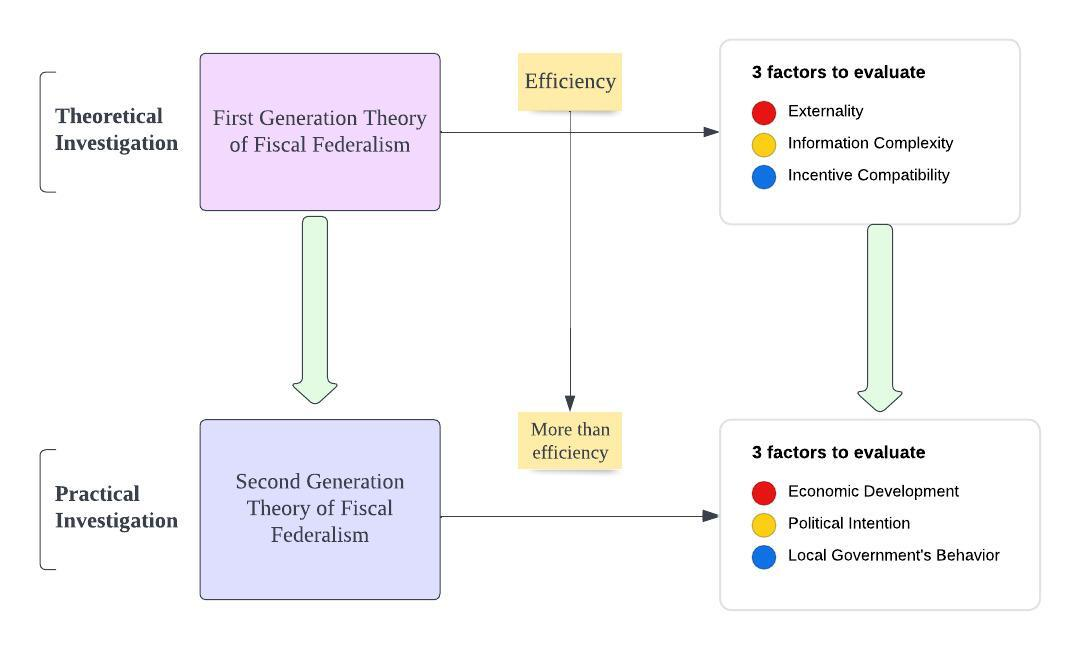
\includegraphics[scale=1]{Chapter-2/Figures/how to evaluate the fiscal federalism.jpeg}
%     \caption[How to evaluate the fiscal federalism]{How to evaluate the fiscal federalism
%         \texttt{} }
%     \label{Figure 2.1}
% \end{figure}

% In summary, as depicted in Figure \ref*{Figure 2.1}, the original research on fiscal federalism constructed a theoretical framework for efficiently providing public goods. In developed countries, particularly in America, scholars have discovered empirical evidence supporting the advantages of this decentralized fiscal structure. However, in developing countries, fiscal federalism has not worked as effectively, leading to the emergence of second-generation theory. This newer approach focuses on the other side of the coin.


\section{National Government's Decision on Engaging Method}
As mentioned in Chapter 1, broadly there are three choices available for national government when dealing with the provision of sublevel jurisdictions' public goods, which are no provision, joint provision and intergovernmental transfer. Based on Volden's \cite{volden2007intergovernmental} dynamic game setting, I expand his setting in three aspects to better investigate governments' behavior. Firstly, I differentiate the intergovernmental transfer into transfer with bare restriction--general transfer and transfer with restriction attached--categorical transfer. Secondly, I assume different kinds of players on subnational level in terms of the resource endowment. Besides, I modified the utility setting for the players in this game compared to Volden's setting. Specifically, my general model setting could be listed as follows.

\subsection{A Dynamic Game Analysis with Complete Information}
The Figure 2.1 demonstrates the extensive form of central and subnational interaction, which is developed based on Volden's game theory model \cite{volden2007intergovernmental}. However, this paper presents a modified version of the game. Departing from Volden's model, by considering two types of players instead of assuming identical subnational governments. Moreover, the paper defines different types of grants and specifies varying restrictions attached to grants. Additionally, the game in this paper incorporates a more comprehensive form of the utility of governments. The game model in this paper can be described in terms of three aspects: player set, behavior set, and utility set.The nuance of the difference between the modal in this paper and Volden's model will be explained in detail in following sections. Besides, the game is assumed to be a dynamic game with complete information, which means the utility for all players in this game is a common knowledge for everyone. In summary, the modified game in this paper offers a more nuanced understanding of the interactions between central and subnational governments.

\begin{itemize}
\item \textbf{Player Set}\\
In the intergovernmental transfer interaction game in this thesis, three players are assumed to exist: the central government $N$, state governments with higher resource endowment $S_h$, and state governments with lower resource endowment $S_l$. The assumption of identical subnational governments is relaxed, as governments with differing resource endowments may have varying preferences, leading to differing reactions to intergovernmental transfers. The player set $P = \{ N, S_h, S_l\}$. For convenience, I defined $i\in \{l,h\}$. \label{player} The difference between $S_h$ and $S_l$ is that the states with higher resource endowment is more productive, possess higher tax bases (GDP).

\item \textbf{Action Set}\\
For central or national government, one available choice for national government is to stay out of the subnational jurisdictions' public goods provision. If national government decide to join the goods provision, there are two available choices, which are 3 ways to join the provision. After deciding how to join the public goods supply, central governmental also need to decide the parameter in different games.  One is to provide the goods directly, in that case,citizens in a specific state enjoy the public goods offered by two level of governments combined.In joint provision game, the national government decide the amount of public goods provided to $S_i$, which are $G_n^i$.

Another one is to offer intergovernmental transfer. In Volden's setting, there are only one kind of intergovernmental transfer. Volden's setting is to compare the difference between intergovernmental transfer and joint provision. I assume there are two kinds of intergovernmental transfer. Transfer to lower level governments are either general transfer $T_g$ or categorical transfer $T_c$ which is more restricted during administrative process and subnational governments cannot use the grants freely as they want to. \label{transfer}

The design of the different transfer is to simulate the difference listed in Table \ref{Table 1.3}. Volden didn't distinguish different kinds of grants in his dynamic game setting. However the restriction may play a role in affecting both national and subnational governments' behavior, thus I differentiate the intergovernmental transfer into different categories in terms of the restriction level to deduce the effect of restriction.

The main goal for the general transfer is to narrow the gap and equalize the resource of different subnational governments. The effect of general transfer has been wildly mentioned in fiscal federalism literatures \cite{buettner2006incentive,lv2018transfer}. I adopted Buettner's design about the amount of general transfer, in which $T_g$ received by government $i$ can be captured as:
$$T_g^i = T_0 - \sigma F_i $$ \label{generaltransfer}
where $\sigma$ captures the central government's intention to equalize the resource in different jurisdictions. A higher $\sigma$ means national government prefer to equalize the resource. For example, compared to US government, OECD central government prefer to set a higher $\sigma$. $T_0$ is the benchmark grants amounts when $S_i$ got zero production output. $F_i$ is the total output in $S_i$. The equalization effect of general transfer in this setting can proven in Appendix C.

Compare with the general transfer, the equity concern is not a main point in categorical transfer game. The role for categorical grants is to affect the policy direction in subnational jurisdictions. By encouraging the spending in specific area, central government may encourage the policy reality to develop in a national-favored direction. The categorical transfer are typically matching transfer, which means the national government pay for specific percentage of the expenditure in specific area and subnational governments pay for the rest. I assume there are two kinds of public goods on subnational level which are productive goods $P$ like roads, railways, and other kinds of infrustracture. Another kind of public good is welfare public goods $W$ like social welfare, salaries for public servants like police officers. Thus $G$ is a public goods matrix and $G=|P\ \  W|$. \label{pgmatrix}
In this thesis I assume matching ratio for productive grants is $m$ and matching ratio for welfare-oriented grants is $n$. Thus the productive and welfare-oriented grants received by subnational government $i$ is:
$$
    \left\{\begin{array}{l}
        T_p^i=m p_i \\
        T_w^i=n w_i
    \end{array}\right.
$$
For convenience, I defined a ration matrix $r=\left|\begin{array}{l}m \\ n\end{array}\right|$. \label{mrmatrix}

To summary, the available action for national government is $$A_N=\left\{N P,\left(J P, G_N^i\right),\left(G T, T_0, \sigma\right),(C T, r)\right\} $$

\newpage


\begin{landscape}
    \begin{figure}[H]
        \centering
        \includegraphics[scale=0.041]{Chapter-2/Figures/tree.jpg}
        \caption[Dynamic Game Tree of 3 players]{Dynamic Game Tree between Central and Subnational Governments
            \texttt{} }
        \label{dynamicgamenoutility}
    \end{figure}
\end{landscape}

\newpage

For subnational governments, they need to decide the public goods $G_i$ they need to provide under no provision game, the public goods $G_s^i$ under joint provision game and public goods $G_i^{gt}$ under general transfer game. I assume subnational government cannot reject the joint provision or general transfer here since it's more like a lump-sum supplement. For categorical grants, I assume subnational governments may choose to reject based on their utility consideration. If subnational governments choose to reject the grants, then the national government is out of the game and the game became a no provision game. If subnational governments decide to accept the grants, then they need to decide the amount of public goods they provide $G_i^{ct}$ based on the matching ration $r$ offered by national government. To summarize, the action set for subnational governments $A_i$ is  $$A_i=\left\{\left(G_i|NP\right),\left(G_s^i |J P \right),\left(G_i^{gt}|G T \right),\left(Accept,G_i^{ct}|C T\right)\right\} $$

\item \textbf{Utility Set}\\
I followed the design of Volden's design but with multiple modifications.

On subnational level, the utility function can be listed as
$$U_i=V_i\left(G_i\right)-t_{si}^{\varepsilon}-\left|y_i-X_i\right|$$
The utility for subnational governments comes from three parts. The first part is the utility from supplying $G$. I assume $V^{\prime}>0, V^{\prime \prime}<0$. The second part is the tax burden $t_{si}$ imposed by subnational government to supply the public goods. $\varepsilon >1 $, which represents the risk averse attitude of the citizens. Basically, subnational governments prefer to maximize the utility of the public goods while control the tax burden blame from citizens. The third part captures the policy direction. I compress the policy direction to a 1 dimension line.Each government has an ideal policy direction on the one dimensional line. $y$ is the actual policy outcome and $X_i$ means the ideal policy outcome for jurisdiction $i$. $|y-X_i|$ captures the distance between the actual policy outcome and the ideal policy outcome of $S_i$. The logic of this term is that the policy direction is typically a compound of both national and subnational impact. For example, central government prefer the policy direction with less negative externality while subnational government focus merely on their own benefits \label{iposition}.

For national government, the utility function can be listed as
$$U_N = \sum_i V_i - \sum_i t_{Ni}^{\varepsilon} - \sum_i \gamma_i|y_i-X_N|$$
The utility for national government comes from three parts as well. For one, the national government cares about the utility from increasing public goods in all subnational jurisdictions combined. The second term still capture the tax burden. The difference is that the national government only take the blame of the national tax $t_{Ni}$. The  third therm also express the utility from policy direction. I add a $0<\gamma_i\leq 1$, which I call bias term, to capture the possible prejudiced bias in national government's decision making process. The thought is, national government may cater aligned subnational jurisdictions' policy preference. Again, I compress the political relationship into a 1 dimensional line. If national government and a subnational government is aligned, such as a blue state under democratic federal, $\gamma_i$ may take a minimal value. If federal and state governments stand in polarized opposite position, then $\gamma_i=1 $ \label{actposition}.

I made balanced budget assumption for both national and subnational governments, which means all tax income all levels of government is all invested into the public goods provision. Suppose the price for public goods in $i$ is $c_i$, and $e_j$ is tax collecting efficiency of player $j \in P$, which is affected by tax collecting ability $a_j$ and tax collecting effort $f_j$, thus I have $e_j=a_j \times f_j$. $a_j$ is decided by multiple factors such as number of administrators, level of salaries in tax administration system, and IT expenditure on equipment \cite{savic2015impact,kiser1994could,aizenman2008collection,mattos2011flypaper}. $f_j$ is a subjective issue and government can decide how much effort they put in tax collection. Based on the balanced budget assumption, I have $\frac{c_i G_s^i}{e_i f_i}=t_i$ or $\frac{c_i G_s^i}{a_i}=t_i$ on subnational level\label{priceandeffort} and $\frac{\sum_i c_i G_n^i}{a_N}=t_N$ on national level.

The modification I made to Volden's dynamic game setting can be summarized in three aspects. Except for the heterogeneous players setting and different transfer setting. One most significant modification is I added fiscal illusion effect and bias factor into the utility function. One fundamental assumption in Volden's assumption is that voters have full information regarding spending at the national and subnational level and they accurately assign credit for goods provision based on those criteria. In another word, governments would consider they can only receive credit for the proportion they supplied. What's more, when national government's role is accomplished through IGT, then "the credit for good provision is divided in proportion to the size of the grant and the total spending by the subnational government" \cite{volden2005intergovernmental}. An extensive assumption is that voters also have full information about the which government should be responsible for the tax raising. Based on these two assumptions, the voters have full information about the merit and fault assignment about the public goods provision. The assertion that voters accurately ascribe electoral credit and blame is based primarily on a federalist perspective on vote-choice \cite{stein1990economic}, and some earlier empirical literature do support this setting \cite{atkeson1995economic}. There are empirical evidence, however, that at least in America, voters ascribe credit and blame for public goods provision inaccurately. For examaple, Carpini and Keeter shows that only 14\% of the interviewees knows about the unemployment rates and 25\% knew about the proportion of the federal spending in terms of the education resource supply \cite{carpini1996americans}. Besides, Gilens indicates that only 12\% of the respondents got correct answer whether the crime rate has risen or declined during last decade \cite{gilens2001political}. Needless to say, a bunch of literature on fiscal illusion talking about voter's inaccurate sense about the price of public goods is also an strong side evidence of the voters' insufficient information \cite{oates1979lump,borge1995lump,turnbull1998overspending}.

Compared with Volden's assumption, I added fiscal illusion consideration into the utility setting. I kept Volden's assumption about the clear assignment on tax burden but I loosen the assumption about credit assignment, which means the voters are clear about the which government is collecting the tax while unclear about which government is providing public goods. Thus the utility from the public goods $V$ is a function of the total amounts of public goods in $i$ $G_i$ which equals national provided amounts to $i$ $G_n^i$ and subnational governments provided amounts $G_s^i$, thus $G_n^i+G_s^i=G_i$. Mathematically, the implication is that the subnational governments have the motivation to welcome the national resource and prefer to be a free rider, which contradict implications in Volden's model--subnational governments have the intention to impede national government resource inflow and increase subnational governments' public goods provision to get more credit. The proof of this free rider motivation is provided in Appendix C.

\subsubsection{No Provision Game}
Under no provision game, subnational government is the only public goods provider. In this game, subnational government would get the utility based on the amount in $i$, which equals to the amounts supplied by subnational government. Also, subnational government take all the blame of raising the necessary tax. Finally, in this game, the subnational government decide the policy outcome exclusively, thus $y=X_i$. In this case, subnational governments' utility is writen as:
$$U_i=V_i\left(G_i\right)-\left(\frac{c_i}{e_i} G_i\right)^{\varepsilon}$$

For national government, they care about the utility from all subnational jurisdictions combined and can still get the utility from voter's public goods consumption, even though they do not supply directly. What's more, national government do not take the blame for tax raising. The cost is that national government has to accept the policy inutility due to the inability to affect the policy direction. To summarize, the utility for national government under no provision game is:
$$U_N=\sum_i V_i-\sum_i \gamma_i\left|X_N^i-X_i\right|$$

\subsubsection{Joint Provision Game}
For joint provision game, both national and subnational government would contribute to the public goods provision directly. For subnational government $i$, they would observe the amount of goods provided by national government $G_n^i$ then decide the amount of goods they would like to provide $G_s^i$. Subnational governments' tax only need to cover $G_s^i$, and I follow Volden's setting that in joint provision game, subnational government decide the policy outcome \footnote{Volden has proven an alternative assumption that $y$ is placed a fixed distance between the national and subnational ideal points in this case yields similar results}. With these three aspects considered, the utility for subnational governments is:
$$U_i=V_i\left(G_i\right)-\left(\frac{c_i}{e_i} G_i\right)^{\varepsilon}$$

National government get the utility from public goods consumption and afford the tax to cover the public goods spending offered by national government in all subnational jurisdictions while not able to impact the policy outcome in $i$. The utility for national government in joint provision game is:
$$U_N=\sum_i V_i-\sum_i \gamma_i\left|X_N^i-X_i\right|$$


\subsubsection{General Transfer Game}
General transfer game means that the subnational government is the direct provider of the public goods with the lump-sum transfer payment from national government. National government only supply grants with no ability to intervene subnational jurisdictions' policy direction. Subnational governments in this game need to decide the public goods supply and policy direction while needless to worry about the full tax burden, thus the utility for subnational government is:
$$U_i=V_i\left(G_i\right)-\left(\frac{c_i}{e_i}\left(G_i-\frac{T_i}{C_i}\right)\right)^{\varepsilon}$$

For national government, the utility comes from the public goods from all jurisdictions combined, while need to take the necessary burden and cannot achieve any impact on subnational jurisdictions policy direction. This setting may be counterintuitive at first--national government seems take the tax burden with no benefits in exchange. The reason lines in the fact that national government cares about the utility of all jurisdiction combined and the marginal effect of one unit product increase in a low endowment subnational jurisdiction should be higher than the marginal effect of same amount product increase in high endowed place, which means national government should be motivated to equalize the public goods provision in different places. The utility for national government in this game is:

$$U_N=\sum_i V_i-\sum_i\left(\frac{T_i}{e_N}\right)^{\varepsilon}-\sum_i \gamma_i \left|X_N-X_i\right|$$

\subsubsection{Categorical Transfer Game}
Under categorical transfer game, subnational governments decide the level of public goods provision level conditional on the matching ratio $r$. Meanwhile, They need to collect tax to partly supply the goods. Also, in this game, subnational governments cannot set the policy position arbitrarily as they want to, national government can affect policy directions by attaching restrictions to the grants. The subnational governments' utility can be summarized as:

$$U_i=V_i\left(G_i\right)-\left(\frac{c_i^{c t}}{e_i} G_i\right)^{\varepsilon}-\left|y_i-X_i\right|$$
where $c_i^{ct}$ is the cost for subnational government conditional on the matching ratio decided by national government, thus I have $c_i^{ct}=(1-r)c_i$

National government care about the public goods provision condition in all subnational area, and need to collect tax to afford part of the public goods. The good thing for national government in this game is that it can affect the policy direction by adjusting the matching ration matrix $r$. The utility of national government in this game can be listed as:
$$U_N=\sum_i V_i-\sum_i\left(\frac{G_i \cdot c_i \cdot r}{e_N}\right)^{\varepsilon}-\sum_i\gamma_i\left|y_i-X_N\right|$$

So the utility for players in player set $P$ based on their actions under different games can be summarized in Table \ref{utilitytable}
% Table generated by Excel2LaTeX from sheet 'Sheet1'
\begin{table}[H]
    \centering
    \caption{Utility of Players under Different Games }
    \begin{tabular}{cp{2.855em}r}
        \toprule
        \multicolumn{1}{p{10.5em}}{Game}                           & Player & \multicolumn{1}{p{14.285em}}\ {Utility}                                                                                \\
        \midrule
        \multicolumn{1}{c}{\multirow{3}[6]{*}{No Provision Game }} & $NG$   & $U_N=\sum_i V_i-\sum_i \gamma_i\left|X_N-X_i\right|$                                                                   \\
        \cmidrule{2-2}                                             & $S_l$  & $U_l=V_l\left(G_l\right)-\left(\frac{c_l}{e_l} G_l\right)^{\varepsilon}$                                               \\
        \cmidrule{2-2}                                             & $S_h$  & $U_h=V_h\left(G_h\right)-\left(\frac{c_h}{e_h} G_h\right)^{\varepsilon}$                                               \\
        \midrule
        \multirow{3}[6]{*}{Joint Provision Game}                   & $NG$   & $U_N=\sum_i V_i-\sum_i\left(\frac{c_N}{e_N} G_N^i\right)^{\varepsilon}-\sum_i\gamma_i\left|X_N-X_i\right|$             \\
        \cmidrule{2-2}                                             & $S_l$  & $U_l=V_l\left(G_l\right)-\left(\frac{c_l}{e_l}\left(G_l-G_N^l\right)\right)^{\varepsilon}$                             \\
        \cmidrule{2-2}                                             & $S_h$  & $U_h=V_h\left(G_h\right)-\left(\frac{c_h}{e_h}\left(G_h-G_N^h\right)\right)^{\varepsilon}$                             \\
        \midrule
        \multirow{3}[6]{*}{General Trasnfer Game}                  & $NG$   & $U_N=\sum_i V_i-\sum_i\left(\frac{T_i}{e_N}\right)^{\varepsilon}-\sum_i \gamma_i \left|X_N-X_i\right|$                 \\
        \cmidrule{2-2}                                             & $S_l$  & $U_l=V_l\left(G_l\right)-\left(\frac{c_l}{e_l}\left(G_l-\frac{T_l}{c_l}\right)\right)^{\varepsilon}$                   \\
        \cmidrule{2-2}                                             & $S_h$  & $U_h=V_h\left(G_{h}\right)-\left(\frac{c_h}{e_h}\left(G_{h }-\frac{T_h}{c_h}\right)\right)^{\varepsilon} $             \\
        \midrule
        \multirow{3}[6]{*}{Categorical Transfer Game}              & $NG$   & $U_N=\sum_i V_i-\sum_i\left(\frac{G_i \cdot c_i \cdot r}{e_N}\right)^{\varepsilon}-\sum_i\gamma_i\left|y_i-X_N\right|$ \\
        \cmidrule{2-2}                                             & $S_l$  & $U_l=V_l\left(G_l\right)-\left(\frac{c_i^{c t}}{e_l} G_l\right)^{\varepsilon}-\left|y_l-X_l\right|$                    \\
        \cmidrule{2-2}                                             & $S_h$  & $U_h=V_h\left(G_h\right)-\left(\frac{c_h^{c t}}{e_h} G_h\right)^{\varepsilon}-\left|y_h-X_h\right|$                    \\
        \bottomrule
    \end{tabular}%
    \label{utilitytable}%
\end{table}%

\subsection{Backward Induction on National Government's Engaging Choice}
The extensive game about national government's engaging method is solved through backward induction. The national government would take the first movement to decide which engaging method to join the public goods provision, then subnational governments decide if they accept or reject national government's decision. Once subnational governments rejected, the game turns into no provision game, which means national government has no role in public goods provision.

So for subnational government, the backward induction analysis gives us that both $S_l$ and $S_h$ won’t accept the categorical transfer unless $U_i|_{CT}>U_i|_{NP}$ otherwise subnational governments would just turn down the grants and supply the public goods without national government's assistance. National governments knows subnational governments' potential motivation to reject the grants. If national government want to make sure that the grants could be accepted, the matching ratio $r$ should be set at a level that could guarantee $U_i|_{CT} > U_i|_{NP}$. Thus I have proposition 1.

\textbf{Proposition 1: One necessary but insufficient condition for national government to choose categorical transfer is $U_i|_{CT} > U_i|_{NP}$}

The compare between $U_i|_{CT}$ and $U_i|_{NP}$ can be analyzed from two angles. Subnational governments either pin down the tax burden then compare the utility increase $\Delta V_i(\frac{G_i}{1-r})$ with the inutility of policy deviation $-|y_i-X_i|$ \footnote[1]{The policy direction is compressed on a one dimension line with $X_N$ and $X_i$ on the two sides, theoretically the actual policy outcome should be somewhere between $X_N$ and $X_i$} or pin down the goods utility $V_i(G_i)$ then compare the tax burden averse decrease $\Delta t=-(\frac{r c_i G_i}{e_i})^\varepsilon$ with policy deviation inutility $-|y_i-X_i|$. In this analysis, I calculate the tax burden with given $V_i^*(G_i)$.

$U_i|_{CT} > U_i|_{NP}$ can be rewritten as $$[1-(1-r)^\varepsilon]( \frac{c_i}{e_i}G_i)^\varepsilon > |y_i-x_i|$$

This equation is a necessary but insufficient condition that the categorical transfer can be achieved by subnational governments. It's decided by multiple parameters including $r,\varepsilon,c_i,e_i$ and the gap between $y_i$ and $X_i$. The implication from the first proposition is that, subnational governments with higher public provision cost, lower tax collection efficiency and may agree to accept the categorical transfer with lower $r$, which represents the price that national government would like to pay, especially when the actual policy outcome is not far away from subnational governments' ideal point. This proposition is different from Volden's proposition that subnational governments should be cautious about the matching ratio $r$ since a higher $r$ means national governments attract more political credit. In this analysis, higher matching ratio $r$ means subnational governments accept the grants easier.

Another natural implication that I list as proposition 2 is on policy gap.


\textbf{Proposition 2: The subnational governments aligned with national government are more likely to accept the categorical transfer}

Aligned governments means national and subnational governments share similar ideas in policy direction thus subnational government bare less policy inutility in categorical transfer game. In extreme circumstances, when national government have exact the same ideal policy point with subnational governments, $X_N = X_i$ and policy inutility became 0.

Once the matching ratio $r$ meets the condition in proposition 1 and subnational governments agree to take the categorical transfer, it's national governments' decision whether the categorical transfer could be executed successfully. National government would evaluate its' utility under different circumstances and compare with categorical transfer, thus I have proposition 3.

\textbf{Proposition 3: Another three necessary but insufficient conditions for national government to choose categorical transfer are $U_N|_{CT} > U_N|_{NP}$,\ $U_N|_{CT} > U_N|_{JP}$\ and\ $U_N|_{CT} > U_N|_{GT}$}

This proposition is a naturally conclusion by backward induction. Except for the necessary condition on the subnational governments side, the national government should have the motivation to choose categorical transfer over no provision, joint provision and general transfer methods. From table \ref{utilitytable} I have:
$$
    \left\{\begin{array}{l}
        \sum_i V_i-\sum_i\left(\frac{G_i \cdot c_i \cdot r}{e_N}\right)^{\varepsilon}-\sum_i\gamma_i\left|y_i-X_N\right| > \sum_i V_i-\sum_i \gamma_i\left|X_N-X_i\right|                                                      \\
        \sum_i V_i-\sum_i\left(\frac{G_i \cdot c_i \cdot r}{e_N}\right)^{\varepsilon}-\sum_i\gamma_i\left|y_i-X_N\right|> \sum_i V_i-\sum_i\left(\frac{c_N}{e_N} G_N^i\right)^{\varepsilon}-\sum_i\gamma_i\left|X_N-X_i\right| \\
        \sum_i V_i-\sum_i\left(\frac{G_i \cdot c_i \cdot r}{e_N}\right)^{\varepsilon}-\sum_i\gamma_i\left|y_i-X_N\right|> \sum_i V_i-\sum_i\left(\frac{T_i}{e_N}\right)^{\varepsilon}-\sum_i \gamma_i \left|X_N-X_i\right|
    \end{array}\right.
$$

Compare $U_N|_{NP}$ and $U_N|_{CT}$, which is the first equation, one necessary but insufficient condition is
$$\sum_i \gamma_i|y_i - X_i| > \sum_i (\frac{G_i c_i r}{e_N})^\varepsilon$$

This equation implies that national government would adjust $r$ such that the tax burden to support the categorical transfer worth the policy direction benefits. This trade off is affect by national government's tax collection efficiency $e_N$, public goods price on subnational level $c_i$. National government with higher tax collection efficiency prefer to



%%%%%%%%%%%%%%%%%%%%%%%%%%%%%%%%%%%%
First thing noticed it that subnational governments has no motivation to reject national government's joint provision or general transfer decision. Rejecting and turning joint provision game or general transfer game to no provision game brings no benefits to subnational governments. For given level of $G_i$, utility for subnational governments under no provision game is obvious less than utility under joint provision and general transfer game $$U_i|_{NP} < U_i|_ {JP}$$  $$U_i|_{NP} < U_i|_{GT}$$ since subnational government can get rid off part of the tax burden while undertake no inutility from public goods level change and policy position deviation. Besides, since it's a complete information game, subnational governments' utility and theoretical choice is transparent for national governments. So for the first three games, the decision is made up purely by national government. The national government would compare the utility within three subgames, which can be listed as:
$$
    \left\{\begin{array}{l}
        U_N|_{NP}=\sum_i V_i-\sum_i \gamma_i\left|X_N-X_i\right|                                                       \\
        U_N|_{JP}=\sum_i V_i-\sum_i\left(\frac{c_N}{e_N} G_N^i\right)^{\varepsilon}-\sum_i\gamma_i\left|X_N-X_i\right| \\
        U_N|_{GT}=\sum_i V_i-\sum_i\left(\frac{T_i}{e_N}\right)^{\varepsilon}-\sum_i \gamma_i \left|X_N-X_i\right|
    \end{array}\right.
$$

The national government would compare the utility  between no provision game and joining the game---either through joint provision or general transfer. Taking the tax burden and joining the game only happens when the total utility after equalizing the public goods provision $\sum_i Vi$ excess the necessary tax burden $\sum_i t_n^i$. Since player $i$ differs in their ability to supply public goods and $V^\prime_l > V^\prime_h$, taking the tax burden and stepping in the subnational level provision to equalize the provision level is not always a irrational behavior for national government.

\textbf{Proposition X: National government tend to provided the general transfer rather than joint provision when the price of public goods for national government provision $c_N$ are relatively higher compared to the cost of subnational government}

This proposition captures the general intuition. For given level of $V_l(G_l)$ and $V_h(G_h)$, national government only need to compare the tax burden term which are $\sum_i\left(\frac{c_N}{e_N} G_N^i\right)^{\varepsilon}$ and $\sum_i\left(\frac{T_i}{e_N}\right)^{\varepsilon}$. To achieve same amount of goods increase $G_N^i$, national government in joint provision game can provide directly while in general transfer game I have $\frac{T_i}{c_i}=G_N^i$.

The compare between $U_N|_{JP}$ and $U_N|_{GT}$ is straight forward, since national government is actually compare $\sum_i c_N G_N^i$ which equals to $\sum_i\frac{c_N}{c_i}T_i$ with $\sum_i T_i$. The implication is that when $\frac{c_N}{c_i}>1$, the national government prefer to choose general transfer rather than joint provision.


